\documentclass{article}
\usepackage[utf8]{inputenc}
\usepackage{amstext}
\usepackage{amsmath} 
\usepackage{mathpazo}
\usepackage{graphicx} 
\usepackage{float} 
\usepackage{caption} 
\usepackage{epstopdf} 
\usepackage{hyperref}
\usepackage{varioref} 
\usepackage{fancyref}
\usepackage[section]{placeins} 
\usepackage{perpage}
\usepackage[margin=1in, paperwidth=8.5in, paperheight=11in]{geometry} 
\MakeSorted{figure} 
\usepackage{natbib}
\usepackage{graphicx}
\usepackage{xcolor}
\usepackage{listings}
\usepackage{minted}
\usepackage{subcaption}
\usepackage{eso-pic}
\usepackage{ amssymb }
\usepackage{tikz}
\usepackage[american]{circuitikz}
\usepackage[font=small,labelfont=bf]{caption}

\title{ENGR2420 Lab 8 : A Simple MOS Differential Amplifier}
\author{Abigail Fry\\ Anusha Datar\\ Vienna Scheyer}
\date{April 22, 2019}

\begin{document}

\maketitle

\section{Experiment One : Voltage Transfer Characteristics}
In this experiment, we constructed a differential amplifier with an nMOS differential pair and a pMOS current mirror. We set the inverting input, $V_2$, to 2.5, 3.5, and 4.5 Volts, and we swept the value of the noninverting input, $V_1$, between 0 Volts and 5 Volts and measured the output voltage of the circuit. We completed this procedure with the bias voltage of the differential pair, $V_b$, set to 0.65 Volts (at threshold) and 1.5 Volts (above threshold).
\begin{figure}[H]
  \begin{center}      
  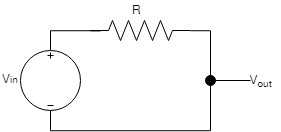
\includegraphics[scale = 0.5]{images/exp1_schematic.jpg}
  \caption{Experiment one schematic.}   
  \label{fig:exp1_schematic}
  \end{center}
\end{figure}

\subsection{Results}
We first measured the value of $V_{out}$ with $V_2$ set to 2.5, 3.5, and 4.5 Volts with $V_b$ set to 0.65 Volts so that the bias current was at the threshold.
\begin{figure}[H]
  \begin{center}      
  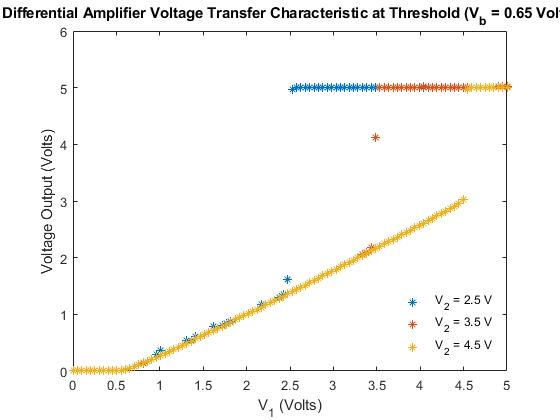
\includegraphics[scale = 0.5]{exp1_plot1.jpg}
  \caption{Voltage transfer characteristic, $V_b$ at threshold.}   
  \label{fig:exp1_plot1}
  \end{center}
\end{figure}
We measured the value of $V_{out}$ with $V_2$ set to 2.5, 3.5, and 4.5 Volts with $V_b$ set to 1.5 Volts so that the bias current was above the threshold.
\begin{figure}[H]
  \begin{center}      
  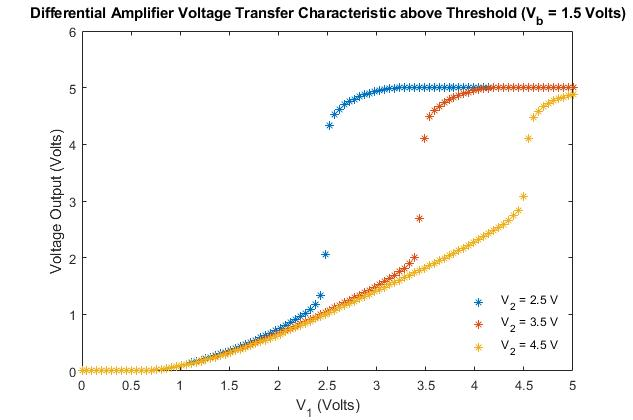
\includegraphics[scale = 0.5]{exp1_plot2.jpg}
  \caption{Voltage transfer characteristic, $V_b$ above  threshold.}   
  \label{fig:exp1_plot2}
  \end{center}
\end{figure}
\subsection{Analysis}
In theory, the differential amplifier's output voltage should remain close to ground when $V_1 < V_2$ until $M_2$ enters the Ohmic region, at which point $V_{out}$ will equal $V$. After $V_1$ exceeds $V_2$, the value of the voltage quickly rails to $V_{dd}$, or 5V.
Our experimental data qualitatively reflects this general pattern in all three cases for both when the bias current is at and when it is above the threshold.  

\subsection{Discussion}
When biased in strong inversion, the circuit displays similar behavior to when biased in weak and moderate inversion, where it quickly rails from low to high Voltage as $V_1$ increases and exceeds $V_2$. While the actual transition is much more gradual in strong inversion than in weak inversion (because the voltage change lags when the bias voltage is above the threshold), the trend is the same. 

\section{Experiment Two : Transconductance, Output Resistance, and Gain}
In this experiment, we measured the differential-mode voltage and output voltage to extract the differential-mode gain.  Next, we measured the output current and output voltage to extract the incremental output resistance.  Finally, we measured the differential-mode voltage and the output current to extract the incremental transconductance gain.  To collect this data, we set $V_{b} = .65$ Volts and $V_{2} = 3.5$ Volts and used the schematic seen in Figure \ref{fig:schm2}.
\begin{figure}[H]
  \begin{center}      
  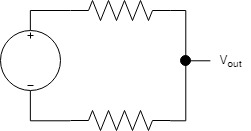
\includegraphics[scale = 0.5]{images/exp2_schematic.jpg}
  \caption{Schematic used to collect experimental data for Experiment 2.}   
  \label{fig:schm2}
  \end{center}
\end{figure}

\subsection{Results}
 First, we plotted the differential-mode voltage vs. output voltage on linear axes.  We found $A_{dm}$ by fitting a line to the steep part of the curve and extracting the slope of that region.  The differential-mode gain for the plot in Figure \ref{fig:DMG2} is $A_{dm} = 138.6165$.  Differential-mode gain does not have units because it is a ratio of voltages.

\begin{figure}[H]
  \begin{center}      
  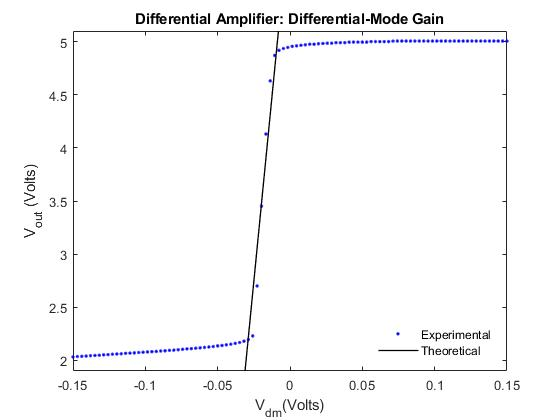
\includegraphics[scale = 0.5]{images/DA_DMG.jpg}
  \caption{Output voltage vs. differential-mode voltage for the MOS differential amplifier }   
  \label{fig:DMG2}
  \end{center}
\end{figure}

Next, we plotted the output current vs. output voltage on linear axes.  We found the output resistance, $R_{out}$, by fitting a linear line to the shallow part of the curve and taking the inverse of the slope.  The output resistance for the plot in Figure \ref{fig:OR2} is $R_{out} = 13.8843 M \Omega$.

\begin{figure}[H]
  \begin{center}      
  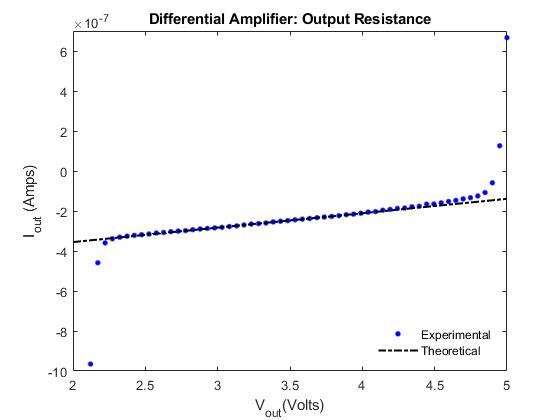
\includegraphics[scale = 0.5]{images/DA_OR.jpg}
  \caption{Output voltage vs. output current for the MOS differential amplifier}   
  \label{fig:OR2}
  \end{center}
\end{figure}

Finally, we plotted the differential-mode voltage vs. the output current.  We found $G_{m}$ by fitting a straight line to where $V_{1} = V_{2}$ and extracting the slope.  The incremental transconductance slope of the plot in Figure \ref{fig:TG2} is $G_{m} = 0.00001287  \mho
$.

\begin{figure}[H]
  \begin{center}      
  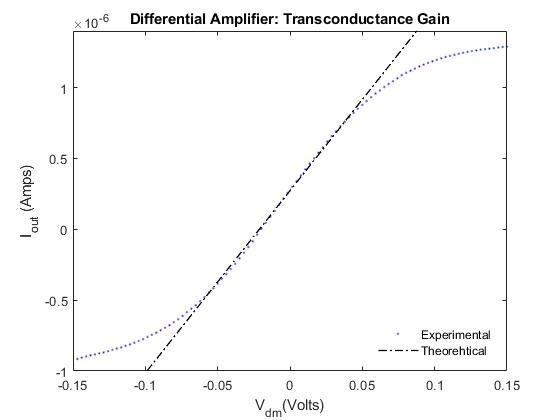
\includegraphics[scale = 0.5]{images/DA_TG.jpg}
  \caption{Differential-mode voltage vs. output current for the MOS differential amplifier}   
  \label{fig:TG2}
  \end{center}
\end{figure}
\subsection{Analysis}
 The equation for incremental differential-mode voltage gain of the circuit can be calculated using the equation below.
\begin{center}
 $A_{dm} = \frac{\delta V_{out}}{\delta V_{dm}} = \frac{\delta V_{out}}{\delta I_{out}} \times \frac{\delta I_{out}}{\delta V_{dm}} = R_{out} \times G_{m}$
   \end{center}
   
 By using the values we extracted in Figure \ref{fig:OR2} and Figure \ref{fig:TG2}, we were able to calculate the value of differential-mode voltage gain.  Then we compared it to the value extracted from Figure \ref{fig:DMG2}.  The extracted value of $A_{dm}$ was 138.6165 and the value calculated was $A_{dm} = 178.7195$.  To quantify the difference between those values we used the percent error equation and found a $28.93 \%$ error between our theoretical (extracted) and experimental (calculated) values. 
 \begin{center}
Percent Error= $\frac{|(Theoretical-Experimental|}{Experimental}\times 100$ 
 \end{center}

\subsection{Discussion}
The percent error between the calculated value and extracted value of $A_{dm}$ for the data we collected was $28.93 \%$.  This percent error makes sense due to the way we extracted $R_{out}$ and $G_{m}$.  We used MATLAB's $polyfit$ function on specific parts of the curves in Figure \ref{fig:OR2} and Figure \ref{fig:TG2} to extract the values.  The range of data points used in the $polyfit$ function were qualitatively found.   This means there is some level of error between experimental and theoretical $R_{out}$ and $G_{m}$.  The error in those extracted values explains why the percent error between the calculated and extracted $A_{dm}$ is almost $30 \%$.

\section{Experiment Three : Unity-Gain Follower}

\begin{figure}[H]
  \begin{center}      
  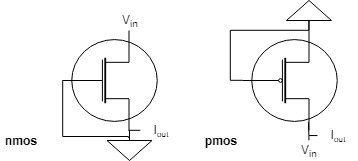
\includegraphics[scale = 0.5]{images/exp3_schematic.jpg}
  \caption{Experiment 3 schematic}   
  \label{fig:exp3_schematic}
  \end{center}
\end{figure}

\subsection{Results}

Figure \ref{fig:unity_gain_follower} shows a plot of the output voltage as a function of the input voltage for our unity gain follower circuit.

\begin{figure}[H]
  \begin{center}      
  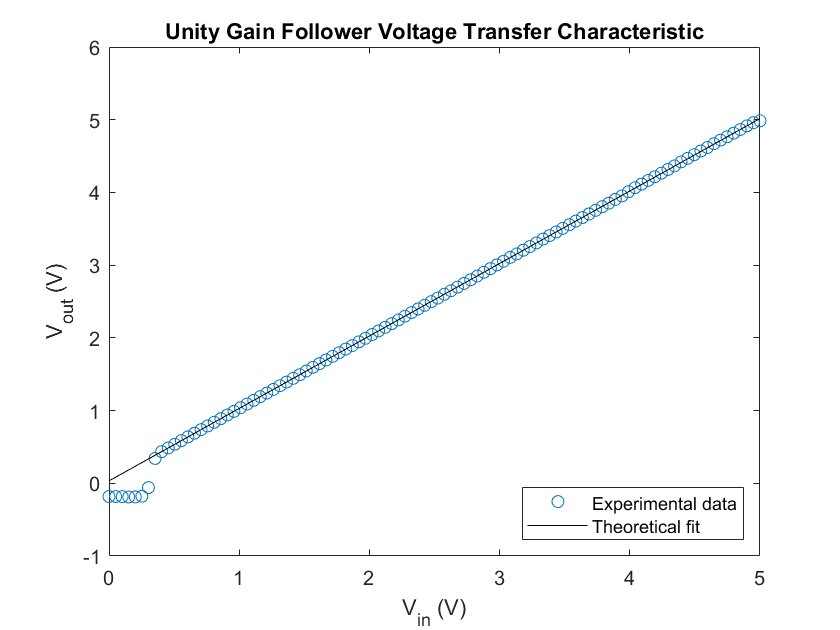
\includegraphics[scale = 0.5]{images/Unity_Gain_Follower.png}
  \caption{Transfer function for unity gain follower circuit.}   
  \label{fig:unity_gain_follower}
  \end{center}
\end{figure}

Figure \ref{fig:offset_voltage} shows a plot of $V_{out} - V_{in}$ as a function of $V_{in}$, which is the offset voltage of the unity gain follower.

\begin{figure}[H]
  \begin{center}      
  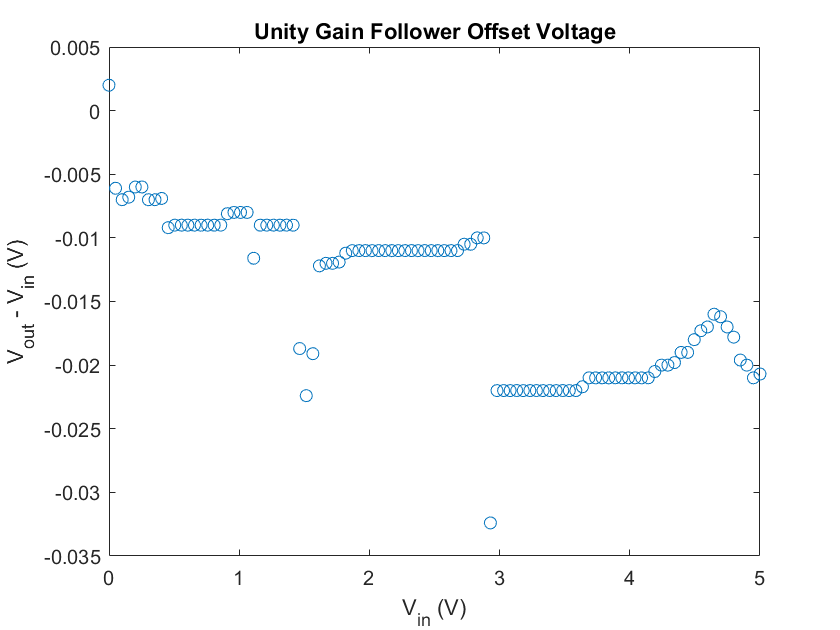
\includegraphics[scale = 0.5]{images/Offset_Voltage.png}
  \caption{Voltage offset for unity gain follower circuit.}   
  \label{fig:offset_voltage}
  \end{center}
\end{figure}

\subsection{Analysis}

For the voltage transfer characteristic, we fit a line to the linear part of the plot using the $polyfit$ function in MATLAB to find the slope, and we found that the slope of the line is 0.9966. We would expect an ideal unity gain follower to have a slope of 1, so we calculated percent error with the following equation:

\begin{center}
    $$Percent \ Error = |\frac{1 - 0.9966}{1}| \cdot 100 = 0.34\%$$
\end{center}

For the offset voltage plot, we plotted $V_{out} - V_{in}$ as a function of $V_{in}$ to see how the unity gain follower differs from unity at each point as we sweep $V_{in}$.

\subsection{Discussion}

The voltage transfer characteristic has an incremental gain of 0.9966, which is quite close to the expected value of 1. We calculated a $0.34\%$ error.

The voltage offset has values that are all close to zero, with the largest value being $-0.0324 V$. The absolute value of the voltage offset increases as $V_{in}$ increases, which suggests that for higher input voltages the unity gain is less accurate. 

\end{document}
